\documentclass[a4paper]{article}
\usepackage[utf8]{inputenc}
\usepackage{a4wide}
\usepackage{url}
\usepackage{alltt}
\usepackage{graphicx}
\usepackage{libs/tex/abbrev_reactive}
\usepackage{listings}%[hyper,procnames]
\lstset{extendedchars=true, language=C++, basicstyle=\scriptsize\ttfamily, numbers=left,
  numberstyle=\tiny, stepnumber=5, numberfirstline=true,
  tabsize=8, tab=\rightarrowfill, keywordstyle=\bf,
  stringstyle=\rmfamily, commentstyle=\rmfamily\itshape}

\let\OldRightarrow=\Rightarrow
\RequirePackage{marvosym}
\let\MarvosymRightarrow=\Rightarrow
\let\Rightarrow=\OldRightarrow
\RequirePackage{wasysym}
\let\Lightning\UnTrucIndefini% Because conflict between ifsym and marvosym
\let\Sun\UnTrucIndefini%
\RequirePackage[weather]{ifsym}


\sloppy

\begin{document}

\title{Par4All Command Line Interface\\
  \texttt{p4a}\\
  ---\\
  HPC Project}

\author{Ronan \textsc{Keryell} \& Grégoire \textsc{Péan}}

\maketitle

\tableofcontents{}

% To automatically build reports from this content:
%%ContentBegin


\section{Introduction}
\label{sec:introduction}

\Apfa is a project aimed at easing code generation for parallel
architectures from sequential source codes written in C or Fortran with
almost no manual code modification required. \Apfa is based on multiple
components, including the \Apips source-to-source compiler framework, and is
developed by \Ahpcp, Mines ParisTech and Institut Télécom. \Apfa is
open source to take advantage of community participation and to avoid
capturing users in a proprietary short-term solution. Specialized target
developments and professional support are also available on demand.

The main goal of a source-to-source compiler is to be naturally
independent of the target architecture details and to take advantage
of the best
back-end tools, such as highly optimized vendor compilers for a given
processor or platform, open-source compilers and tools, high-level
hardware synthesizers, \Acuda or \Aopencl compilers for \Agpu. At the same
time, some architectural aspects can be expressed or generated in
special source constructs to capture architectural details when needed
(\Asimd or accelerators intrinsics). The source-to-source aspect makes
\Apfa \emph{de facto} interoperable with other tools as front-end
or back-end compilers to build complete tool chains.

\texttt{p4a} is the basic script interface for users who are
not interested in \Apips details but wish to produce parallel code from
user sources.

This script can take C or Fortran source files and generate \Aopenmp or
\Acuda output to run on shared memory multicore processors or
\Agpu, respectively.

The output is created in files with the same name as the original ones, with a
\emph{.p4a} extension added before the original extension. The generated files are
extracted from a temporary \texttt{\emph{x}.database} directory that can be kept
for later inspection (standard practice for \Apips usage).

This script can also be used to call a back-end compiler such as
\texttt{gcc}, \texttt{icc} or \texttt{nvcc} to generate a binary
executable. Compiler and preprocessor options can be passed directly
to the back-end compiler via the script.

A CMake build infrastructure can be automatically generated to ease
compilation by the back-end.

The \Apfa documentation is available from \url{http://www.par4all.org} and
more specifically, this document can be found in \Apdf from
\url{http://download.par4all.org/doc/simple_tools/p4a/p4a_script.pdf}

Since \Apfa is a large project in progress with continuous updates,
users should refer to the current release notes and the general
documentation on
\url{http://www.par4all.org} for updates on
the current status and limitations of the tools.

This project is funded through various research projects : French ANR
FREIA, European ARTEMIS SCALOPES, French Images and Network TransMedi@,
French System@tic OpenGPU, French ANR MediaGPU, European ARTEMIS SMECY.


\section{Examples and use cases of \protect\texttt{p4a}}
\label{sec:examples}

\subsection{Automatic parallelization with OpenMP generation}
\label{sec:autom-parall-with}

To generate \Aopenmp code from a Fortran program, use:
\begin{verbatim}
p4a --openmp example.f
\end{verbatim}
which produces output in the file \texttt{example.p4a.f}. Since this is
the default
behavior, the \verb/--openmp/ option can be omitted. The compilation
process automatically data-parallel \emph{do}-loops into
\Aopenmp parallel loops with the correct pragmas and with the privatization of
scalar variables.


\subsection{Automatic parallelization with CUDA generation}
\label{sec:autom-parall-with-1}

To generate from a C program source a \Acuda program that is also compiled
into an executable, use:
\begin{verbatim}
p4a --cuda example.c -o e
\end{verbatim}
which produces an \texttt{example.p4a.cu} \Acuda program source and an
\texttt{e} executable that will run on a \Agpu. The \Agpu accelerator
support relies on a small \Apfa Accel interface that connects to the
\Acuda infrastructure. Data-parallel loops are automatically transformed
into \Acuda kernels that execute on the \Agpu. \emph{Ad
  hoc} communications between the host memory and the \Agpu memory are
generated to enable kernel execution.

To generate an \Aopenmp emulation executable of \Agpu-like accelerated
code (for debugging or if a \Agpu is not available), use:
\begin{verbatim}
p4a --accel --openmp example.c -o e
\end{verbatim}
which produces a \texttt{e} binary executable file with its
corresponding \texttt{example.p4a.c} program source. This \Aopenmp
emulation of \Acuda with memory transfer may be helpful for debugging
since there is no longer emulation mode in recent versions of \Acuda.

The advantage of the source-to-source approach is that the
generated code can be further improved manually or used as a starting
point for other
developments. When compiling the \Apfa Accel generated code,
different preprocessor symbols can be defined according to the expected target:
\begin{itemize}
\item \verb|P4A_ACCEL_CUDA| preprocessor symbol, the source is to be
  compiled as \Acuda;
\item \verb|P4A_ACCEL_OPENMP| preprocessor symbol, the source is to be
  compiled as \Aopenmp or sequential emulation code.
\end{itemize}

The native compilation scheme is to generate allocation on the \Agpu for
each parallel loop nest, transfer to the \Agpu the data needed for the
computation, launch the kernel and copy back the results from the \Agpu.
For iterative algorithms for example, some data can often remain on the
\Agpu between kernel calls because they are not touched by the host. For
this, there is an optional optimization that can be used with the
\verb|--com-optimization| option: a static interprocedural data-flow
analysis keep track of data movement and allocation to remove redundant
communications and allocation, leading to great performance improvements. This
options supposes that you make use of static and/or C99 VLA array, it would 
be broken by malloc'ed arrays in parallel section.

Parallelization of some functions can be avoided by using
\texttt{-{}-exclude-modules=\emph{regex}}. This is preferable when the
parallel part is not compute-intensive enough to compensate for
the overhead of transferring data and launching a kernel. In this
case, parallel execution is more expensive than sequential execution. 
The option \texttt{-{}-select-modules=\emph{regex}} is complementary to the
previous one and can be useful to speedup the process by focusing on specific
functions.

There is also an option to exclude some files from the back-end
compilation, for example, to use libraries that have been optimized
already. To use this option,
the program is analyzed by providing stubs definitions in a source
file. The stubs definitions
are dummy function definitions that have similar global memory
effects to the original functions so that \Apips global
interprocedural analysis can proceed correctly. For subsequent compilation
in the back-end stage, this file is skipped with \verb|--exclude-file|, then
the dummy calls are replaced with the real library functions by linking
them with \texttt{-l} or compiling them with \verb|--extra-file|.

Look at section~\ref{sec:options} for a full list of options.


\subsubsection{P4A Accel runtime tweaking}
\label{sec:p4a-accel-runtime}

To ease code generation and portability, \Apfa does not directly generate
direct \Acuda code and instead generates calls to functions and
macrofunctions defined in the P4A Accel runtime.

There are many parameters that can be changed to better suit a given
application on a given target.

In the case of \Acuda generation, you can pass flags to the \texttt{nvcc}
back-end compiler with the \verb|--nvcc-flags=...| option.

For example:
\begin{itemize}
\item to debug the output with \texttt{cuda-gdb}, use
  \verb|--nvcc-flags="-g -G"|;
\item to optimize the \Acuda code use \verb|--nvcc-flags=-O3|;
\item  to generate code to Fermi board use
  \verb|--nvcc-flags="-gencode arch=compute_20,code=sm_20"|;
\item to generate code to both Tesla \& Fermi board use
  \verb|--nvcc-flags="-gencode arch=compute_10,code=sm_10 -gencode arch=compute_20,code=sm_20"|.
\end{itemize}

The P4A Accel runtime itself can be debugged with
\verb|--nvcc-flags=-DP4A_DEBUG| to output debugging messages around all
the \Acuda kernels invocations, such as: {\scriptsize
\begin{verbatim}
 P4A: Calling 2D kernel "p4a_kernel_wrapper_0" of size (8192x8192)
 P4A: Creating grid of block descriptor "P4A_grid_descriptor" of size 16x8192x1
 P4A: Creating thread block descriptor "P4A_block_descriptor" of size 512x1x1
 P4A: line 43 of function p4a_kernel_launcher_0 in file ".../parameterized_kernel.p4a.cu":
 P4A: Invoking kernel (p4a_kernel_wrapper_0, P4A_grid_descriptor, P4A_block_descriptor) with (i, j, array)
\end{verbatim}
}

Some time measurements can be displayed by defining
\verb|--nvcc-flags=-DP4A_TIMING|.

A runtime some error message such as:
\begin{verbatim}
CUTIL CUDA error : P4A CUDA kernel execution failed :
too many resources requested for launch
\end{verbatim}
signifies that there are not enough registers to run all the requested
threads in a block. To remove this error,
relaunch \texttt{p4a} with a
\verb|--nvcc=-DP4A_CUDA_THREAD_MAX=384| or less, instead of the default
value of 512 threads per block.

The maximum number of threads in a block for 1D
kernels can be selected with a
\verb|--nvcc-flags='-DP4A_CUDA_THREAD_PER_BLOCK_IN_1D=...'|

For 2D kernels, \verb|P4A_CUDA_THREAD_X_PER_BLOCK_IN_2D| and
\verb|P4A_CUDA_THREAD_Y_PER_BLOCK_IN_2D| can be set in the same way. For
efficiency reasons, on nVidia \Agpu, the threads are first allocated along
the $X$ dimension (the \emph{warp} dimension) until the
\verb|P4A_CUDA_THREAD_X_PER_BLOCK_IN_2D| limit is reached, and then along
the $Y$ dimension. In the current revision, parallel loop nests are
limited to the 2 outer parallel dimensions to cope more easily with \Acuda
\Agpu hardware limitation. The inner selected parallel loop is mapped onto
the $X$ \Agpu dimension, which must have a sufficient number of processors
for the level of parallelism.

For more tweaking, look at the \Apfa Accel runtime source on
\url{http://download.par4all.org/doc/Par4All_Accel_runtime/graph} or
directly in the \Agit repository.

\subsection{Automatic task generation for the SCMP architecture}
\label{sec:scmp}

To generate an application for the SCMP architecture from a C program, use:
\begin{verbatim}
p4a --scmp example.c
\end{verbatim}
The tasks must have been previously identified with labels prefixed by
\texttt{scmp\_task\_}\footnote{Advanced users can change this prefix
  by changing the \Apips \texttt{SCALOPES\_KERNEL\_TASK\_PREFIX}
  property.}.

The compiler generates two directories:
\begin{itemize}
\item \texttt{applis/}  contains the automatically generated control task file (\texttt{.app} file);
\item \texttt{applis\_processing/project\_name/} contains the buffers
  description header file (\texttt{scmp\_buffers}), the
  \texttt{*.mips.c} task files and a \texttt{Makefile.arp} to compile
  and build the final application.
\end{itemize}

Some further post-processing may be required to limit the memory
footprint of the generated application. This process has not yet been
automated.

\section{\protect\texttt{p4a} full option list}
\label{sec:options}

The basic usage is \texttt{p4a [\emph{options}] <\emph{source files}>}

The following documentation is automatically generated from the
\texttt{p4a} source code.

\input{p4a-help}


\section{\protect\texttt{p4a} architecture}
\label{sec:p4a-architecture}

The global architecture of \Apfa is given on
figure~\ref{fig:transit_intestinal}.

\begin{figure}
  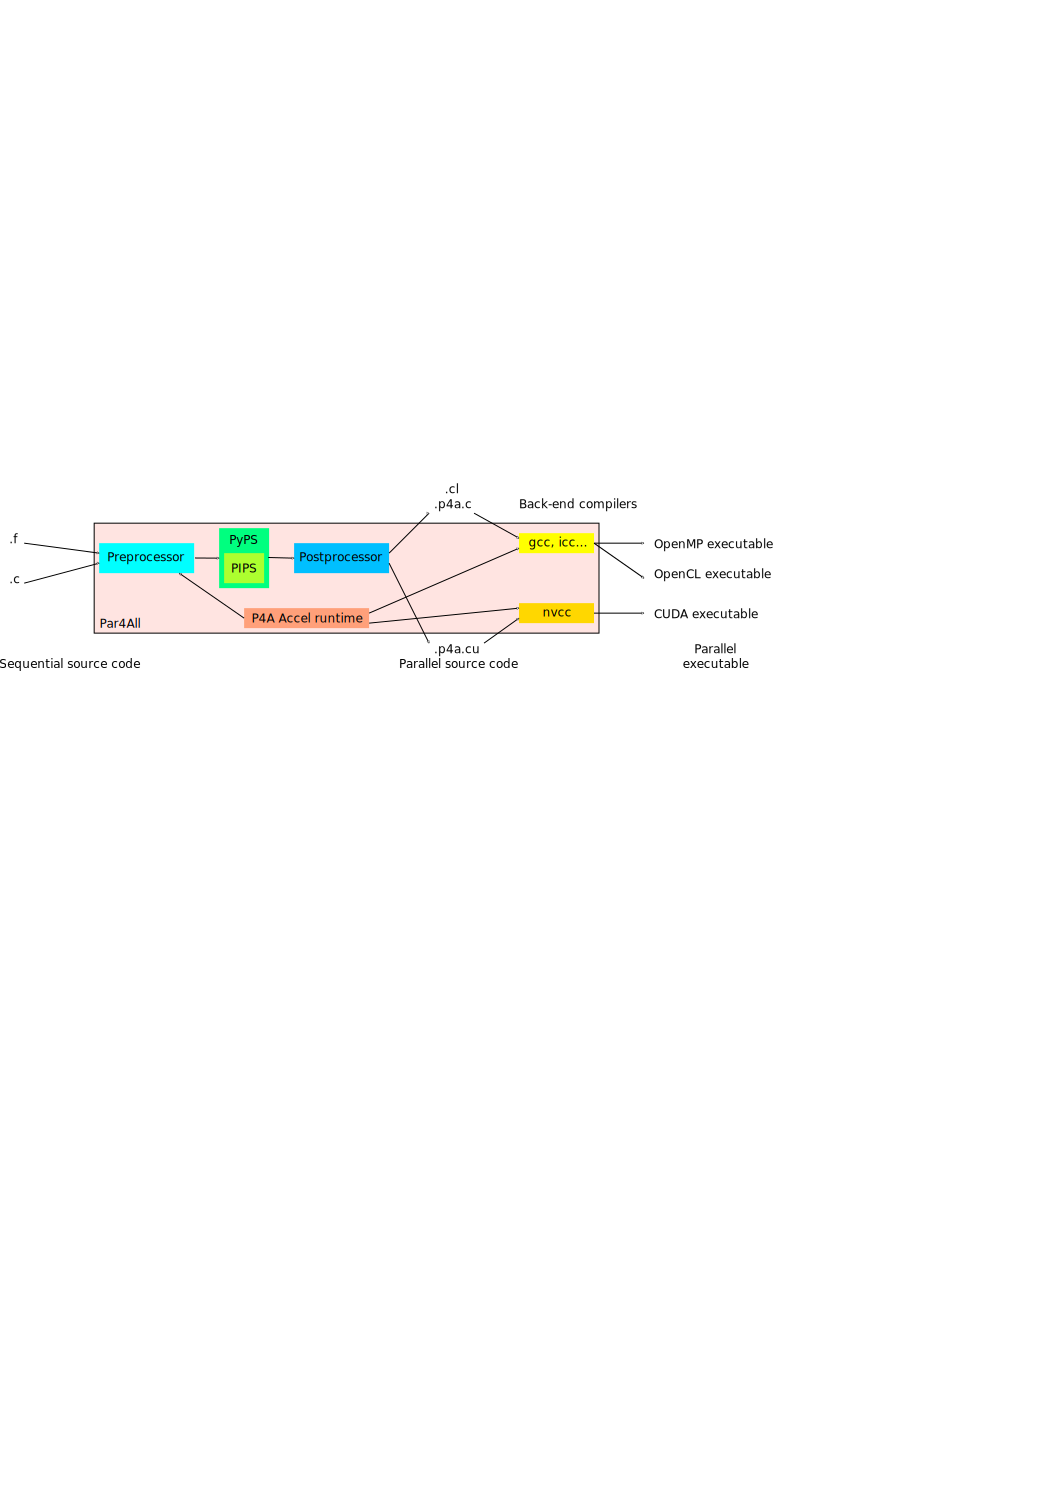
\includegraphics[width=\hsize]{p4a_work_flow}
  \caption{Intestinal view of \texttt{p4a}.}
  \label{fig:transit_intestinal}
\end{figure}

From the high-level user point of view, the sources follow this journey:
\begin{itemize}
\item the source files pass through the preprocessor of
  \Apips. C source files also pass through
  \verb|p4a_recover_includes| to instrument the
  \verb|#include| processing for later recovering;
\item the preprocessed files pass through a splitter that creates
  one file per function and a compilation unit file that keeps track
  of all the file-global declarations;
\item each function file or compilation-unit file can be parsed on
  demand according to the \Apyps script;
\item a predefined \Apyps program applies many different \Apips phases on
  the code and regenerate the transformed sources;
\item \verb|p4a_recover_includes| is applied again as a post-processor
  to recover most of the \verb|#include| work;
\item the sources are postprocessed by
  \verb|p4a_post_processor.py| to cope with some of the special syntax
  (\Acuda, \Aopencl...) that can not be directly represented in \Apips;
\item the generated final files are copied to the final directory;
\item if requested, the final target back-end compilers are called to
  produce the parallelized executable program.
\end{itemize}


\section{\protect\texttt{p4a} extension for advanced users}
\label{sec:p4a-extension}

The main work flow in \texttt{p4a} is
defined in \verb|p4a::main| from \verb|p4a.py|:
\begin{itemize}
\item load \Apyps;
\item normalize user source file names;
\item call \verb|p4a_process| to do the code transformation with \Apyps;
\item generate \texttt{Cmake} configuration files if asked;
\item build the final executable with a \verb|p4a_builder|.
\end{itemize}

Most of the interesting work is done inside \verb|p4a_process::process|,
in another process (if not using the \verb|--no-spawn| option) so that
\texttt{p4a} can do some \Apips output message post-processing. The
interesting steps are:
\begin{itemize}
\item \verb|p4a_process::processor::parallelize|;
\item \verb|p4a_process::processor::gpuify| generate \Agpu-like code if the
  \verb|--accel| option is set;
\item \verb|p4a_process::processor::ompify| if \Aopenmp output
  is requested;
\item \verb|p4a_process::processor::save| regenerate the source files from
  \Apips internal representation with \verb|unsplit()|, call the
  \verb|#include| recovering, call the \verb|p4a_post_processor.py| if
  \Agpu code generation asked. The generated files are saved to
  their destinations with the correct file extensions.
\end{itemize}

The advantage of the \texttt{p4a} script is that it is a simple tool that
behaves well on simple programs but also allows the advanced user to go
further within a practical infrastructure.
To specialize \texttt{p4a} to the needs of particular users, it is
possible to execute
arbitrary Python code at the start of \texttt{p4a} execution with the
\verb|--exec| option.

The given code is executed in the \verb|main| function of the \verb|p4a|
script just after option parsing but just before option handling and the
call to \verb|p4a::main|.

The \verb|p4a.execute_some_python_code_in_process| Python variable can be
used to inject code at the beginning of \verb|p4a_process::process|.
The code can access local variables of the script but not change
them and can both access and change global symbols, such as global
\texttt{p4a} methods.
\verb|p4a_process::default_properties| contains the \Apips properties used
in \texttt{p4a}.

Below are some examples of \texttt{p4a} customization that change the
behaviour of \Apyps inside \texttt{p4a} by importing some modules for more
practical modifications.

First an example to change only one method:
\lstinputlisting[language=Python]{p4a_process_inject.py}

Another example showing how to change a whole class as well:
\lstinputlisting[language=Python]{p4a_process_inject_class.py}


%%ContentEnd

\end{document}


%%% Local Variables:
%%% mode: latex
%%% ispell-local-dictionary: "american"
%%% End:

